\documentclass[11pt]{article}
\usepackage{fontspec}
\usepackage{ctex}
\usepackage{CJKutf8}
\usepackage{graphicx}
\graphicspath{{figures/}}
\usepackage[left=1.25in,right=1.25in,top=1in,bottom=1in]{geometry}
\begin{document}
		\begin{titlepage}
			\centering
			\vspace*{1.75cm}
			\quad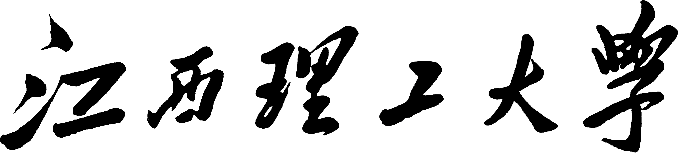
\includegraphics[width=10.53cm,height=1.64cm]{1}\\
			\vspace*{5em}
			{\fontsize{19pt}\baselineskip《科研方法论》课程报告}
			%\textbf{《科研方法论》课程报告}
			\vskip 5cm
			\fontsize{19pt}\baselineskip
			\makebox[30mm]{学\qquad 院:}
			\underline{\makebox[75mm][c]{ 信息与工程学院}}\\
			\vskip 0.9cm
			\makebox[30mm]{专\qquad 业:}
			\underline{\makebox[75mm][c]{信息与通信工程}}\\
			\vskip 0.9cm
			\makebox[30mm]{学\qquad 号:}
			\underline{\makebox[75mm][c]{ \LARGE 6120210299}}\\
			\vskip 0.9cm
			\makebox[30mm]{姓\qquad 名:}
			\underline{\makebox[75mm][c]{谢唯嘉}}\\
			\vskip 2cm
			时间:\LARGE{2022}年2月23日		 
		\end{titlepage}
\newpage

\section{学习做研究}
\subsection{如何进入一个研究领域}

进入一个领域最简单也是最有效的办法是找一本这个领域最早的论述专著或教材。当你把这个领域的基本概念的内涵以及相互之间的关系搞清楚了之后,再去读这个领域的论文,你就会因为心中有数而能够很好地把握了。这种工作必须要先做,不可以在网上乱搜论文,否则,你会感到:看了20篇文章,对这个领域的认识还没有形成,这些概念自相矛盾。由此认识还算幸运,有的人恐怕被偏见所引导,还不知道,这是最可怕的。

\subsection{如何得到导师的指导}

研究生期间应该开始培养独立研究的能力,所以导师一般采用宽松管理。除了几个重要的时间点老师会主动的找学生以外,其余时间都需要学生主动与老师联系。导师是否真的成为你的导师,完全要看你自己的努力,同届的几个学生,可能会得到不同数量的指导,这并不是导师厚此薄彼,而是平时交流频度和质量决定的。因此,我的建议是:

1)自觉地将阶段性成果向导师汇报,听听导师的建议,老师也许会从研究方法和细化问题的角度帮助你反思,更多的时候是为你提供其它的数据来源和支持(人力、物力)。

2)认真地完成老师交给你的看似与你的论文并无关系的事情。老师往往根据对你的直觉认识,认为你合适做什么事情而分配给你一些工作,也许别人对你也是这个印象,也许这是你自己都没有察觉到的你的优势。认真地有意识地发展这方面的知识和技能,会使你成为一个有特长的人。

3)和老师的接触有正式和非正式两类,正式的需要预约,真的是有事情要讨教。非正式的包括路过老师的门口,打个招呼,闲聊两句。有时候正是这种无心插柳,可能带来了很多的机会和资源,也可以得到一些意想不到的指点。

4)不要唯导师命是从,有时候导师分配给你某个任务也有投石问路的意思,是因为想发掘你的潜力。所以多和导师交流你的兴趣和想法,可以方便老师分配给你所想要的机会,做你想做的事情。

5)记住,任何时候研究中遇到问题,都可以直接进入导师办公室,寻求帮助,即使你认为是你自己的问题。这样做的另外一个好处是,让老师知道你是因为有问题而进展停滞,而不是忙其它事情去了。

\subsection{研究生期间要学什么}
我认为研究生期间学生应该学三件事情:

1)建立合理的知识结构:尽量广地涉猎学科基本知识,尽量深地了解所研究领域的方方面面、过去和现在

2)掌握独立研究的方法和技能:尽量多的学习各种研究方法,熟练掌握研究过程和步骤

3)学会写论文:写论文不仅是训练表达能力,更是训练思维的逻辑性,论文体例虽是八股,但却是整理思路、与他人沟通的有效结构,不可不尊重

如果能够按照这三条要求自己,毕业后做不做本专业,并不重要,因为你的研究素质已经建立了,做什么事情都没有问题了。

研究生不能同大学生一样学习,不能主要靠听课做笔记。如果学习的重点是听课,这样的学习就有点类似大学生的学习了。我觉得研究生就是要更多与老师对话,不能只听老师讲,而要更多地与老师讨论,要敢于主动地讲自己的学习体会。所以我希望你们能够多讲,尤其在专业课上,你们要多讲。譬如英帝国史这门课每个学期每个人可以争取主讲几个问题,如讲三个问题。我给你们列了许多小专题,提供了书目,你们可以选择一些问题来探讨。你们讲,我来听,我们互相讨论。研究生学习要有研讨气氛,要有经常性的、体制性的讨论课。讲完后,你们就每一个问题写一篇文稿,我可通过批改文稿,进一步发现你们在探讨这些问题中存在的不足和值得注意的地方。

关于学习做研究的问题,这主要包括两个方面:一、培养研究素质,二、学会写论文。我先简单谈一谈培养研究素质的问题,然后再重点讲如何写论文。

研究素质是什么?不同的学者可能有不同的看法。就我们这个学科而言,我认为研究素质主要包括以下因素。第一,科学态度。科学态度不是与生俱来的,必须认真培养,关键是培养我们在研究中认真负责一丝不苟的精神。第二,献身精神。从事深度学习研究,就像从事其他任何科学研究一样,要有一种为科学研究而献身的精神,要热爱我们的研究事业,要有潜心从事这项工作的意志。没有献身精神,当然做不好科研工作。只想拿一个学位,那是很难学好做研究的。要拿学位,这一点可以理解,但我们读书,是为了自己获得真才实学。有了真才实学将来不论做什么工作,都是有用的。当然学位也是要的,但关键的是学问而不是学位。第三,查阅收集学术信息、资料的能力。青年学生要从事学术研究,就要培养能熟练地掌握查阅搜集学术信息、资料的能力。例如学习与研究深度学习,就得了解国内外有关这个专业的基本情况,了解有关资料情况。像我们在赣州地区学习,至少要大致了解赣州地区有关深度学习的中英文资料,熟悉与专业密切相关的主要图书馆,了解馆藏情况。这就需要经常去图书馆。我们这个专业不需要到田间考察,到工厂调研,但要去图书馆,去图书馆就是我们的调查研究。熟悉有关图书馆的情况是我们学习的一部分。今天,网络飞速发展,掌握网上查阅信息的技巧是非常必要的。第四,处理资料的能力。搜集的资料会越来越多,怎样安排它们也是一门学问。各学科各个研究人员的方式可能会有所不同,但总的原则是要有条理,便于记忆,便于查阅。第五,对资料的鉴别意识与鉴别能力。我们在使用研究资料时不能拿着就用,要有意识鉴别一下,材料是否可靠,什么样的材料更有价值。读书时,也不是拿着什么书就通读到底。有的书翻一翻即可,有的书则需认真读。区别哪些书翻一翻即可,哪些书得认真读,也不是一件容易的事,青年学生不是一下子就能做到这一点的,需逐渐培养这种能力。还有一点就是要学会使用计算机,能比较熟练地进行文字处理。

研究生学习的一项基本内容是学会写论文,如何撰写论文,我的体会是:写论文有四个基本步骤。第一,大量阅读有关著述,掌握有关资料;第二,从中发现问题,确定自己要写的论文的大致题目;第三,根据自己确定的选题,有目标地搜集能够搜集到的一切资料;第四,撰写论文本身。

在写作之前,我们往往得做一件十分重要的工作,即专有名词的确定。在这一点上,对某些外文资料中的专有名词要译成中文。如何译,有时要费很大力气。还有,英文著作中的学术概念,我们要准确理解,有些概念在使用时,需赋予新的含义,不能拿来就用,要着力建立自己的概念体系和思想体系。

下面我想重点谈一下撰写论文的具体过程。第一,熟悉搜集到的有关资料,对某些问题形成基本看法,再列出一个写作提纲。第二,根据写作提纲回过头来重新阅读有关资料,并运用相关资料阐述史实和自己的看法,构成一篇文稿。现在对你们来说都需要用计算机来处理文稿,这样要方便得多,尤其便于修改。第三,初稿写成后,要进行基本的文字修改。像我们的英帝国史专业,由于所引用的资料几乎全是英文,而且多半是档案文件材料,比一般著作更难读懂。在写初稿应用材料时,实际上同时在做翻译工作。在写初稿时,为了保证思路流畅,对于翻译文字不能仔细推敲,所以初稿写成后,文字很粗糙。那么在修改时,一项基本任务就是反复推敲原文材料,看自己的理解和中文表达是否准确,是否符合原文。在写初稿时要简要注明材料的出处,便于修改时查对,即使有些地方在正式发表时不一定需要做注释,但在初稿时却要标明,以便自己修改和查对。这样进行文字修改后,形成第二稿,打印出来。

在第二稿的基础上,还需认真进行一次文字修改。修改文字时,一个非常重要的任务是,避免文字的洋味。我们使用的是英文材料,由于英文和中文在语法结构上有很大区别,文字表达上也很不相同,在运用材料时,往往容易出现带有洋味的中文。这是我写作过程中容易犯的毛病,也是青年学生容易犯的通病。我们要尽量用标准的中文写作。在用英文材料时,我更强调的是准确,而不是文字的优美。当然,文字要尽可能优美,但不能以牺牲准确为代价。在第二稿时,一般要认真做注释,按通常的学术标准做注释。做注释也是一门学问,必须认真对待,好好学习,不能采取无所谓的态度,这涉及到是否采取科学态度的问题。注释做好了,便于自己和读者查阅。在做注释上,有两点我想特别提出来,一是引用别人的观点,不管是正式发表的还是尚未正式发表的,都要注明。二是自己从哪里看到的材料,就注明从哪里引用的,不能弄虚作假。例如,有些档案材料,自己并没有亲眼看过,而是从别的作者的著述中看到的,就不能像自己亲自看了一样作注,应写明转引自或直接注明引自某著述。做了注释,这样可以形成第三稿。

第三稿打印出来后,进一步进行文字修改,把所有表达不清的地方说清楚,把所有赘句、赘词、赘字全都删掉,使文字向简洁优美靠拢,思路清晰,逻辑严密。当然,文字功夫的提高是没有止境的。要不断学习。冰冻三尺,非一日之寒。所以第三稿还要回过头来认真查对每个注释是否有误,是否有不符合标准的地方。对于人名、地名、时间等,没有百分之百的把握时,就得查对。

经过这样修改之后,文章已基本定型。此时,我的经验是打印一稿,放一段时间,然后再最后定稿。定稿时有两大任务:一、进一步进行文字润色,尽量做到简明易懂:二、如感到对某些史料不踏实,还要进行查对,直到每一处都准确可靠为止。下一步才能把文稿付诸发表。
\section{人体姿态识别综述}
\subsection{单人姿态估计}
2015 年之前的方法都是回归出精确的关节点坐标( x,y ),采用这种方法不好的原因是人体运动灵活,模型可扩展性较差。本文主要是2015年之后人体姿态识别的发展综述。(1)遮挡问题,这个问题恐怕是最难的,也是必须要解决的(2)速度过慢。(3)仅仅有二位的姿态是不够的,目前也有这一类的研究,关于直接从2d到3d的姿态进行直接估计。这一点是未来发展的趋势。

单人姿态估计性能评价指标:MPII单人数据集,LSP数据集和FLIC数据集。通过对比这三个数据集的PCK值来评价模型好坏。评价指标为PCK(Percentage of Correct Keypoints)即关键点正确估计的比例,计算检测的关键点与其对应的groundtruth 间的归一化距离小于设定阈值的比例,FLIC中是以躯干直径作为归一化参考,MPII中是以头部长度作为归一化参考,即PCKh。

\textbf{发展历程:}

1.《Flowing ConvNets for Human Pose Estimation in Videos》ICCV 2015

2015 年 flow convnet 将姿态估计看作是检测问题,输出是 heatmap。用相对于AlexNet更深的CNN网络进行人体姿态估计,提高关节点定位的鲁棒性,利用temporal提高精度。其创新点在于从卷积神经网络的 3 和 7 层提取出来,再经过卷积操作,称之为空间融合模型,用来提取关节点之间的内在联系;同时使用光流信息,用来对准相邻帧的 heatmap 预测。最后使用参数池化层,将对齐的heatmap 合并成一个 scoremap(置信图)。

网络pipeline:对于当前帧t,输入它的相邻的前后n帧。利用全卷积神经网络(Spatial Net + Spatial Fusion Layers)对每一帧输出一个预测的heatmap。再利用光流信息将这些heatmap扭曲到当前帧t。之后将warped的heatmap合并到另一个卷积层中,该层学习如何权衡来自附近框架的扭曲的heatmap。最后使用集合热图的最大值作为人体的身体关节。

评测数据集:FLIC数据集,对于wrist(手腕)和elbow(肘部)的平均PCK可以达到92\%,可以做到实时性,速度为5fps。但是该方法对于pose的估计范围有限,只是半身的关节点,并不是全身的身体骨骼点。

2.《Convolutional Pose Machines》CVPR 2016

2016 年提出的 CPM 方法具有很强的鲁棒性,之后的很多方法是基于此改进的。CPM 的贡献在于使用顺序化的卷积架构来表达空间信息和纹理信息。网络分为多个阶段,每一个阶段都有监督训练的部分。前面的阶段使用原始图片作为输入,后面阶段使用之前阶段的特征图作为输入,主要是为了融合空间信息,纹理信息和中心约束。另外,对同一个卷积架构同时使用多个尺度处理输入的特征和响应,既能保证精度,又考虑了各部件之间的远近距离关系。

网络输入彩色图像(绿色ori image)。以半身模型为例,分为四个阶段(stage)。每个阶段都能输出各个部件的响应图(蓝色score),使用时以最后一个阶段的响应图输出为准。center map(绿色)是一个提前生成的高斯函数模板,用来把响应归拢到图像中心。 第一阶段是一个基本的卷积网络1(白色convs),从彩色图像直接预测每个部件的响应。半身模型有9个部件,另外包含一个背景响应,共10层响应图。第二阶段也是从彩色图像预测各部件响应,但是在卷积层中段多了一个串联层(红色concat),把以下三个数据合一:

阶段性的卷积结果为46*46*32纹理特征 , 前一阶段各部件响应为46*46*10 空间特征 ,中心约束(46*46*1) ,串联后的结果尺寸不变,深度变为32+10+1 = 43。第三阶段不再使用原始图像为输入,而是从第二阶段的中途取出一个深度为128的特征图(feature image)作为输入。同样使用串联层综合三种因素:纹理特征+空间特征+中心约束。 第四阶段结构和第三阶段完全相同。在设计更复杂的网络时(例如全身模型),只需调整部件数量(从10变为15),并重复第三阶段结构即可。

该论文的主要训练细节有三:1. 数据增强:对原始图片进行随机缩放,旋转,镜像2. 标定:在每个关节点的位置放置一个高斯响应,来构造响应图的真值。对于含有多个人的图像,生成两种真值响应,一是在每个人的相应关节位置,放置高斯响应。二是只在标定的人的相应关节位置,放置高斯响应。3. 中继监督,多个loss:如果直接对整个网络进行梯度下降,则输出层在经过多层反向传播会大幅度的减小,解决方法就是在每个阶段都输出一个loss,可保证底层参数正常更新。

评测数据集:MPII,LSP,FLIC,在MPII数据集上的total PCKh是87.95\%(如果加上LSP数据集作为训练,将达到88.52\%),在LSP数据集上的PCKh是84.32\%(如果加上MPII数据集作为训练,将达到90.5\%),在FLIC数据集上的PCK@0.2分别是elbows(97.59\%),wrist(95.03\%)。

3.《Stacked Hourglass Networks for Human Pose Estimation》ECCV 2016

本文使用全卷积网络解决人体姿态分析问题,截至2016年5月,在MPII姿态分析竞赛中暂列榜首,PCKh(误差小于一半头高的样本比例)达到89.4\%。与排名第二的CPM(Convolutiona Pose Machine)1方法相比,思路更明晰,网络更简洁。该论文体现了从模块到网络再到完整网络的设计思想。

使用的初级模块称为Residual Module,得名于其中的旁路相加结构。Residual模块提取了较高层次的特征(卷积路),同时保留了原有层次的信息(跳级路)。不改变数据尺寸,只改变数据深度。可以把它看做一个保尺寸的高级“卷积”层。

4.《Adversarial PoseNet: A Structure-aware Convolutional Network for Human Pose Estimation》ICCV 2017

采用的GAN的方法,效果比之前的state-of-the-art仅仅提升了零点几个百分点。基本上到hourglass之后的方法都是一些微调,虽然理论都不太一样,但是准确度提升不大。

5.《Learning Feature Pyramids for Human Pose Estimation》ICCV 2017

模式识别的方法,pictorial structures以及loopy 结构,这些方法都是基于HOG 特征。后来是神经网络,最早的是deepPose,是使用回归坐标点的方法。坐标点难以训练学习,后来的方法都是将点做了高斯转换得到score map。同时,还会用到多尺度获得丰富特征。

多尺度特征Hourglass无疑是最成功的。但后面的多种网络结构对这这一基础网络做了调整和优化,有更好的效果。比如这篇,将使用金字塔模型。不是普通的金字塔,而是组合了residual模型和Inception的金字塔,所以计算要求不高。
\subsection{多人姿态估计}
1.《DeepCut: Joint Subset Partition and Labeling for Multi Person Pose Estimation》 CVPR 2016

2016 年的 deepcut,采用自顶向下的方法,先用 CNN 找出所有候选的关节点,将这些关节点组成一幅图,对图中的节点进行聚类,从而判断各个节点属于哪一个人,这是一个优化问题;同时,对各个点进行标记,分类属于身体的哪一部分;两者结合输出姿态估计结果。

Deepercut 是在 deepcut 的基础上使用 resnet 进行检测提高精度,使用 image conditioned pairwise ,能够将丰富的候选节点进行压缩,提升速度和鲁棒性。

评测数据集:deepcut,对于单人姿态估计,在LSP数据集上的PCK达到87.1\%,在MPII数据集上的PCK达到82.4\%(可见,适用于多人的姿态估计方法和纯粹的单人姿态估计方法的准确率还有所差距);对于多人姿态估计,在WAF数据集上mean PCP达到84.7\%,在MPII多人数据集上AP 达到 60.5\%,速度非常慢。

DeeperCut:和deepcut的评测数据集相同,这里主要针对多人来看,其准确率和速度都有所提升,尤其是速度方面。

2.《ArtTrack: Articulated Multi-person Tracking in the Wild》CVPR 2017

2017年的ArtTrack的作者也是DeeperCut 的第一作者,是将人物姿态估计用到了视频跟踪里面,本文的贡献是利用现有的单帧姿态估计模型作为基础框架,但是速度却明显加快,这种加快主要通过以下两种方式来进行:(1)通过简化和稀疏身体部位的关系图,使用进来的方法进行快速的推理;(2)不加载用于前馈神经网络上的大规模计算量,这些神经网络是为了检测和关联同一人的身体关节。模型仍然是采用 top-down 的方法,即先用 Resnet 检测出body part proposal,然后再根据关联和空间信息将他们归为不同的人。

同时,本文也提出一种 top-down/bottom-up 的模型,即 top-down 部分是用来对人体做一个粗略的估计,之后再用bottom-up 进行精确调整,使得预测的关节点位置更准确。

评测数据集:WAF数据集和MPII Video Pose数据集,相应有所提升。

3.《Realtime Multi-Person 2D Pose Estimation using Part Affinity Fields》CVPR 2017

2017 年的 Part Affinity Fields(PAF)能够针对多人做到实时检测,它采用的却是自底向上的方法,网络框架分为两路;一路使用 CNN,根据置信图进行关节点预测,另一路使用CNN 获得每个关节点的 PAF,PAF 可以看作是记录 limb 位置和方向的 2D 向量。两路进行联合学习和预测。最后就是如何将这些节点两两连接不重复,这转换为图论问题。

评测数据集:COCO 2016关键点检测数据集+MPII multi-person benchmark。对于MPII多人pose,本文无论是准确度还是精度上都有质的飞跃,其相比于DeeperCut的速度快了4万多倍,准确度也有几个百分点的提升。可以做到实时,每帧只需要50毫秒,即20FPS。

4.《Mask R-CNN》ICCV 2017,FAIR,Kaiming He

2017年何凯明的Mask R-CNN,Mask R-CNN 是用于目标检测分割的框架,即对一张图片,既输出图片中已有的目标,还能为每一个实例生成一个高质量的分割掩码。mask RCNN是在 faster R-CNN 的基础上,在每一个 RoI 都增加一个预测分割的mask,这和分类以及 bounding box 回归是并行的一条分支。它的训练简单,仅仅比 faster RCNN多一点计算开销。它易于泛化到多个任务上,例如人体姿态估计。在不加任何的 trick的情况下,在COCO 数据集上超越其他的方法。因此准确度方面基本上已经是state-of-the-Art。

应用到pose estimation,将分割系统中的目标改为K个one-hot,m*m的二进制mask。准确率比COCO 2016 冠军高0.9个点,速度达到5 FPS。

5.《Towards accurate multi-person pose estimation in the wild》CVPR 2017

Google的人体姿态估计,多数时候在论文中简写为G-RMI。

论文采用top-down的结构,分为两个阶段: 第一阶段使用faster rcnn做detection,检测出图片中的多个人,并对bounding box进行image crop; 第二阶段采用fully convolutional resnet对每一个bonding box中的人物预测dense heatmap和offset; 最后通过heatmap和offset的融合得到关键点的精确定位。

6.《Associative Embedding:End-to-End Learning for Joint Detection and Grouping》

论文提出了一种single-stage,end-to-end的关节点检测和分组方法,这不同于以往的multi-stage的关节点检测方法,在MPII和COCO数据集上达到新的state-of-the-art的效果,超越最近的Mask RCNN和Google GMI。从人体姿态估计方法上属于bottom-up的方法,即先检测关节点,再对关节点进行分组。在COCO测试集上mAP达到0.655。

7.《RMPE: Regional Multi-Person Pose Estimation》ICCV 2017,SJTU,Tencent Youtu

文章的写作背景是单人姿态估计的方法不能用在多人上面,而多人姿态估计方法虽然效果不错,但是太慢了(485 seconds per image)。它对于多人姿态估计的方法采用传统的自顶向下的方法,即先检测人,再识别人体姿态。检测使用的是SSD-512,识别人体姿态使用的是state-of-the-art的Stacked Hourglass方法。致力于解决对于imperfect proposal,通过调整,使得crop的单人能够被单人姿态估计方法很好的识别,从而克服检测带来的定位误差。

目前的人体检测方法会产生两个主要问题:定位错误,以及多余的检测结果,尤其是SPPE (singal person pose estimation)。这篇文章就是为解决这个问题而来的,提出了RMPE方法。包括了三个模块:Symmetric Spatial Transformer Network (SSTN)用于在不准确的bounding box下仍能提取准确的单个人的范围,这是组合到SPPE里面的。NMS是处理多余的候选框的,它是采用了新的距离量测的方法来计算姿态的相似度,且是数据驱动的,不是预先设定的。PGPG用于增多训练样本。

\subsection{相关数据集}
1.LSP(Leeds Sports Pose Dataset)

地址:http://sam.johnson.io/research/lsp.html

样本数:2K

关节点个数:14

全身,单人

2.FLIC(Frames Labeled In Cinema)

地址:https://bensapp.github.io/flic-dataset.html

样本数:2W

关节点个数:9

全身,单人

3.MPII(Max Planck institut informatik)

地址:http://human-pose.mpi-inf.mpg.de/

样本数:25K

关节点个数:16

全身,单人/多人,40K people,410 human activities

4.MSCOCO(Common Objects in Context)

地址:$\texttt{http://cocodataset.org/\#download}$

样本数:>= 30W

关节点个数:18

全身,多人,keypoints on 10W people

5.AI Challenge

地址:https://challenger.ai/competition/keypoint/subject

样本数:21W Training, 3W Validation, 3W Testing

关节点个数:14

全身,多人,38W people

6.3D数据集:

在数据处理阶段,3D比2D复杂很多。2D人体姿态识别在dataset和model方面都比3D成熟,2Dmodel也有很多户外,自然界的dataset,但是3D的dataset几乎都是indoor的。因为3D标注、识别的复杂,所以需要大量的传感器,摄像头去采集数据。收集了几个最近看到的数据集分享给大家。

7.Human3.6M数据集   

 Human3.6M数据集有360万个3D人体姿势和相应的图像,共有11个实验者(6男5女,论文一般选取1,5,6,7,8作为train,9,11作为test),共有17个动作场景,诸如讨论、吃饭、运动、问候等动作。该数据由4个数字摄像机,1个时间传感器,10个运动摄像机捕获。
 
8.CMU Panoptic dataset

该数据集是CMU大学制作,由480个VGA摄像头,30+HD摄像头和10个Kinnect传感器采集。

9.MPI-INF-3DHP        

该数据集由Max Planck Institute for Informatics制作,详情可见Monocular 3D Human Pose Estimation In The Wild Using Improved CNN Supervision论文。
\end{document}